\documentclass{article}
\usepackage{graphicx}

\title{How do you Define a Canadian?}
\author{Xie, Michael,\\
CANADIAN HISTORY SINCE WORLD WAR 1 - CHC2D Credit 1.0 - 3}
\date{\today}

\begin{document}
\maketitle
\section{Introduction}
What is the essence of a Canadian? What are the defining characteristics that sets Canadians apart from other nationalities?
In this article, we will explore various perspectives on what it means to be Canadian and attempt to define the core attributes that embody Canadian identity.
We will start simple, investigating simple defintions like geography and citizenship, then move to more complex ideas like culture, values, and social norms.

\section{Geographical Definition}
\textbf{Defintion 1:} \\\\
\textit{
A Canadian is someone who resides (as a permanent resident or citizen) within the geographical boundaries of Canada.
} \\\\

This definition is straightforward and easy to apply. However, it does not incorperate the cultural and social aspects that contribute to Canadian identity.
\section{Value Definition}
\textbf{Defintion 2:} \\\\
\textit{
A Canadian is someone who embodies the core values of Canada, such as multiculturalism, politeness, and respect for diversity.
} \\\\

\textit{Canada} is a society pricipled on diversity and perspectives. between 1951 and 2021, the percentage of the immigrant population increased from 14.7\% to 23.0\%.
\begin{figure}[ht]
    \centering
    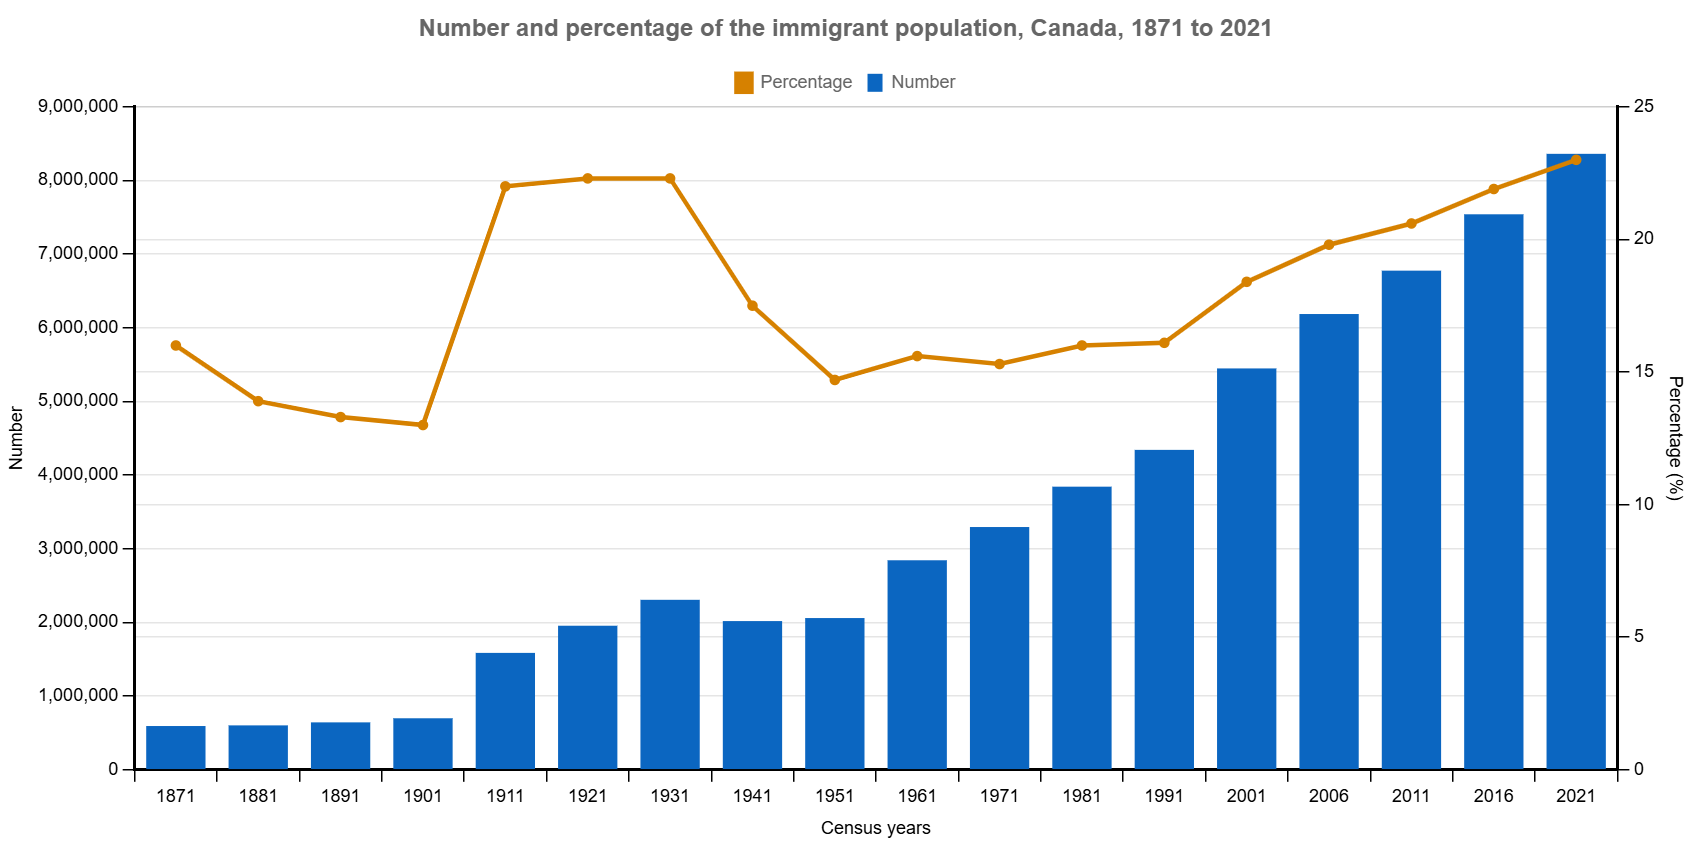
\includegraphics[width=\textwidth]{fogs_2021A000011124_9_2.png}
    \caption{Number and percentage of the immigrant population, Canada from 1871 to 2021}
\end{figure}

Canada depends on it's immigrant population to grow and thrive.
Incorperating the values of multiculturalism and respect for diversity into the constitution and social norms of Canada
fundementally maintains the stabilty of the state.
Canada reached a \textit{tipping point} in the late 90's where the immigrant population reached a critical mass,
Forcing a shift from the standard model of a "unifying culture" to a "mosaic" model where multiple cultures coexist and are celebrated.
The stabilty of this model is hard to maitain, as it requires a high level of respect and tolerance between different cultural groups.
However, it is this very respect and tolerance that defines the Canadian identity.

This is the essence and beauty of Canada. A country that is stable through diversity, able to balance all ideals.
It is important for us to remember that this balance is delicate and requires constant effort to maintain. 
Although history has shown that such approaches always failed in the long run, We must strive to uphold these values and maintain the delicate balance that defines us as Canadians.
This comes at a time of great political termoil, with \textit{internal conflict} rising in Canada, and civil unrest quietly buliding.
My hope is that we can all come together and remember what it means to be Canadian, and work towards a better future for all.\\\\

\textit{Step back from the audious flames of the present, and consider the lessons of the past. The arc of history is long, and the patterns shown bring Canada to a crossroads. We must choose our path wisely, for the future of our nation depends on it.}
\section{Conclusion}
In conclusion, defining a Canadian is a complex task that goes beyond simple geographical or legal definitions.
It involves a deep understanding of the values, culture, and social norms that shape Canadian identity.
Ultimately, being Canadian is about embracing diversity, respecting others, and contributing to the collective well-being of the nation.
\end{document} 